\chapter{Local Administrator Password Solution}
\section{Einleitung}
Local Administrator Password Solution (LAPS) ist eine Lösung von Microsoft.
Mit LAPS werden die Passwörter der lokalen Administratoren, welche auf allen Windows Geräten vorhanden sind, zufällig und unterschiedlich voneinander gesetzt.
Zusätzlich werden die Paswörter in einem gewissen Zeitraum automatisch neu gesetzt.\\

Dies verhindert, dass ein Angreiffer auf weitere Systeme vordringen kann, wenn ein lokales Administratorpasswort komprimiert ist.
Die Passwörter sind in einem Attribut auf dem Computer Objekt im Active Directory hinterlegt.
Zugriff auf dieses Attribut haben nur berechtigte Benutzer.

\subsection{Voraussetzungen}
Um LAPS einsetzen zu können, wird eine Active Directory benötigt mit allen Windows Geräten als Computer Objekte.

\section{Installation}
Die Installation ist in drei Schritte unterteilt.
\begin{enumerate}
    \item Zuerstes wird LAPS via Group Policy auf allen Windows Geräten installiert.
    \item Danach wird das Active Directory für LAPS vorbereitet. Das Active Directory braucht zwei zusätzliche Attribute auf den Computer Objekten um die Passwörter verwalten zu können.
          \begin{itemize}
              \item \textbf{ms-Mcs-AdmPwd}: Speichert das Administrator Passwort in Klartext.
              \item \textbf{ms-Mcs-AdmPwdExpirationTime}: Speichert den Zeitpunkt für den Passwortwechsel.
          \end{itemize}
    \item Zum Schluss wird LAPS per Group Policy aktiviert.
\end{enumerate}

\subsection{Installation via GPO}
LAPS kann auf der \href{https://www.microsoft.com/download/details.aspx?id=46899}{Webseite von Microsoft}\footnote{Link: https://www.microsoft.com/download/details.aspx?id=46899} heruntergeladen werden.
Die .msi Datei muss in einem freigegebenen Netzlaufwerk platziert werden, auf welches alle Windows Geräte Zugriff haben.
Zum Beispiel auf dem Domain Controller unter:
\begin{lstlisting}
    C:\Windows\SYSVOL\sysvol\<Domain>
\end{lstlisting}
Dieses Verzeichnis ist Standardmässig auf Domain Controllern freigegeben.\\

Im Group Policy Management muss eine neue Group Policy erstellt werden, welche mit der OU verknüpft ist, die alle Windows Geräte enthält.
\begin{figure}[H]
    \centering
    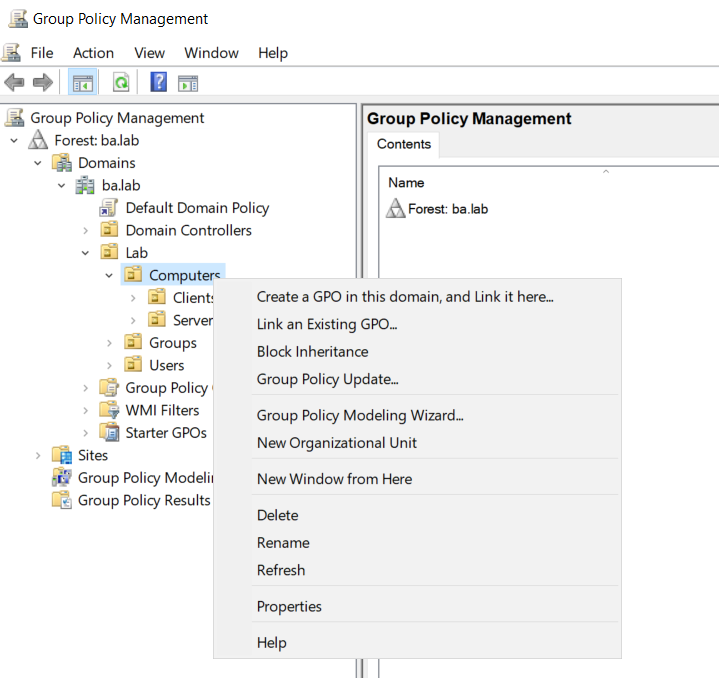
\includegraphics[width=0.7\linewidth]{../img/LAPS/GPO-Create-New.png}
    \caption{Neue GPO für LAPS Deployment}
\end{figure}

Mit \textbf{Rechtsklick $\rightarrow$ Edit} kann die neue Group Policy bearbeitet werden.
Unter \textbf{Computer Configuration $\rightarrow$ Policies $\rightarrow$ Software Settings $\rightarrow$ Software installation} kann mit \textbf{Rechtsklick $\rightarrow$ New $\rightarrow$ Package\dots} eine Datei ausgewählt werden, welche installiert werden soll.
Hier muss man die zuvor im freigegebenen Netzlaufwerk abgelegte Installationsdatei auswählen.\\
\begin{minipage}{0.5\linewidth}
    \begin{figure}[H]
        \centering
        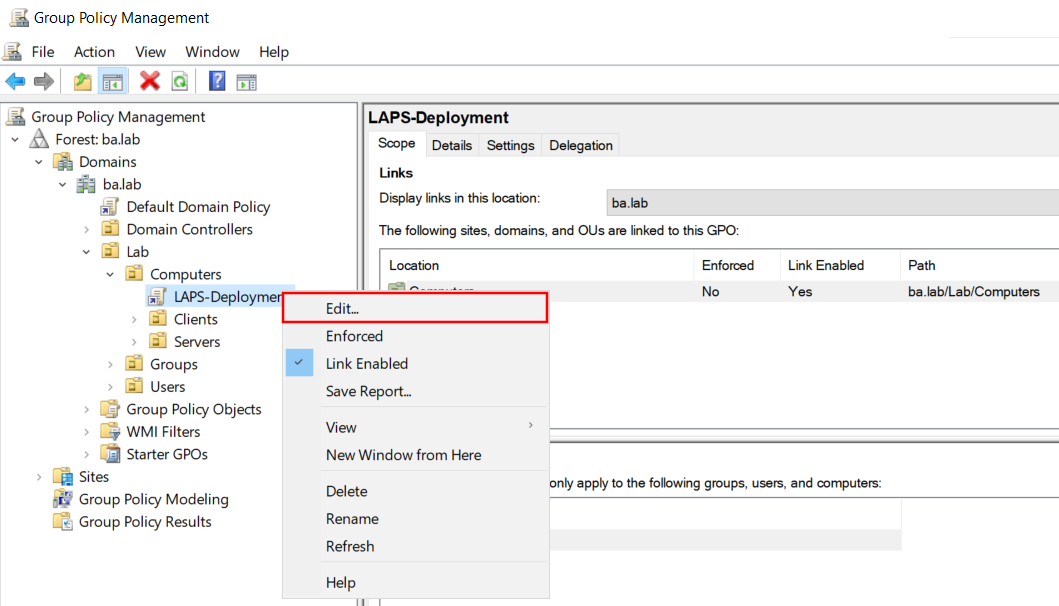
\includegraphics[width=\linewidth]{../img/LAPS/GPO-Edit-Deployment.png}
        \caption{GPO für LAPS Deployment bearbeiten}
    \end{figure}
\end{minipage}
\begin{minipage}{0.5\linewidth}
    \begin{figure}[H]
        \centering
        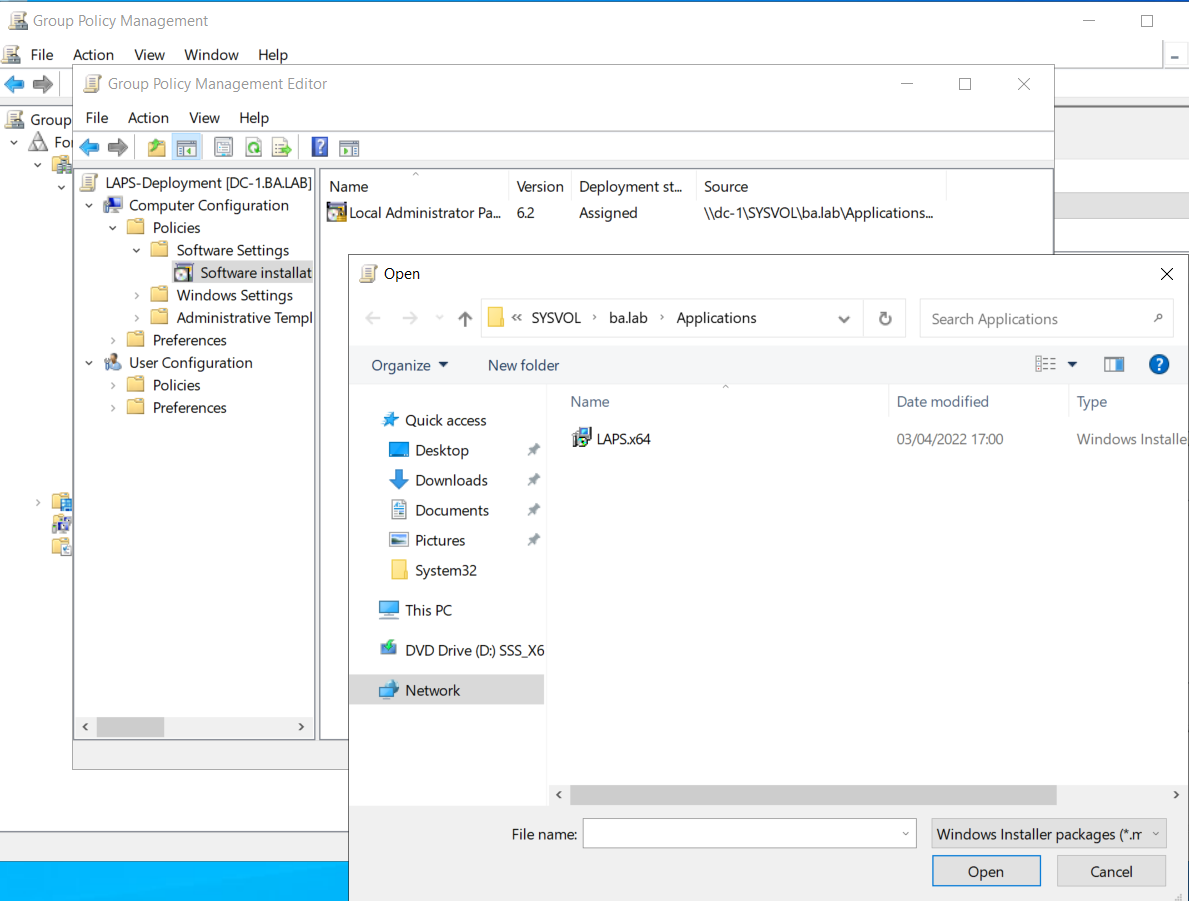
\includegraphics[width=\linewidth]{../img/LAPS/GPO-Edit-Deployment-2.png}
        \caption{LAPS Installationsdatei auswählen}
    \end{figure}
\end{minipage}\\

Die Group Policy kann nun geschlossen werden.
LAPS wird beim Einloggen auf den jeweiligen Geräten installiert.

\subsubsection{Domain Controller}
Auf dem DC sollte man LAPS von Hand installieren.
Bei der manuellen Installation müssen die zusätzlichen Features installiert werden.
Diese sind das GUI, das Powershell Modul und die GPO Richtlinien.

Dazu die Installationsdatei ausführen und alle Features installieren.
\begin{figure}[H]
    \centering
    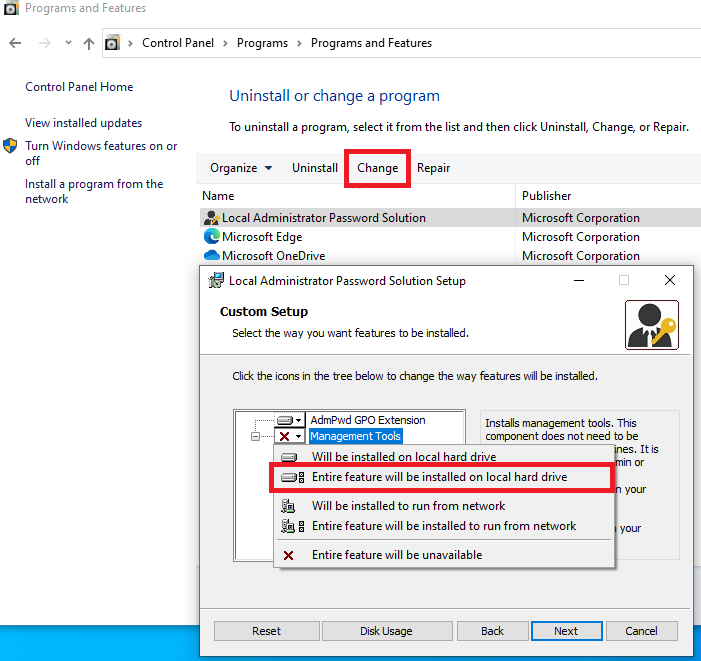
\includegraphics[width=0.7\linewidth]{../img/LAPS/laps-ui-install-2.png}
    \caption{LAPS manuelle Installation}
\end{figure}


\subsubsection{LAPS GUI für Admins}\label{subsubsec:Laps-Gui}
Über die GPO wird auf den Computern LAPS ohne GUI installiert.
Mit dem GUI kann das Passwort von beliebigen Windows Geräten in der Domäne abgefragt werden.\\

In der Programmliste in den Systemeinstellungen auf LAPS klicken und im Balken auf \textbf{Change} klicken.
\begin{figure}[H]
    \centering
    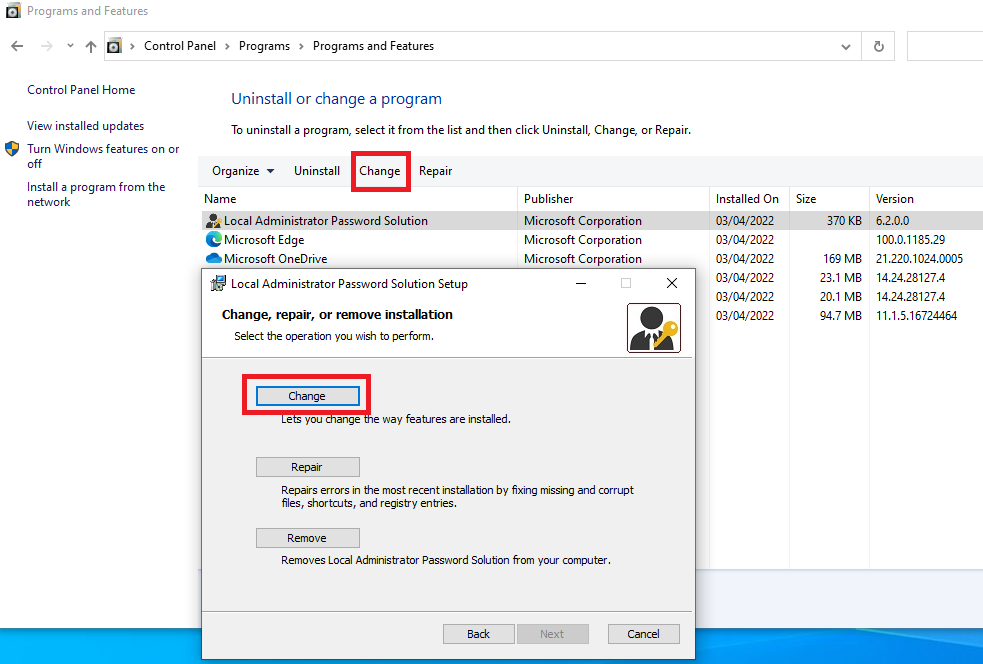
\includegraphics[width=0.7\linewidth]{../img/LAPS/laps-ui-install.png}
    \caption{LAPS GUI Installieren 1}
\end{figure}

Das \textbf{Management Tools} Feature auswählen und dem Installationsprozess folgen.
\begin{figure}[H]
    \centering
    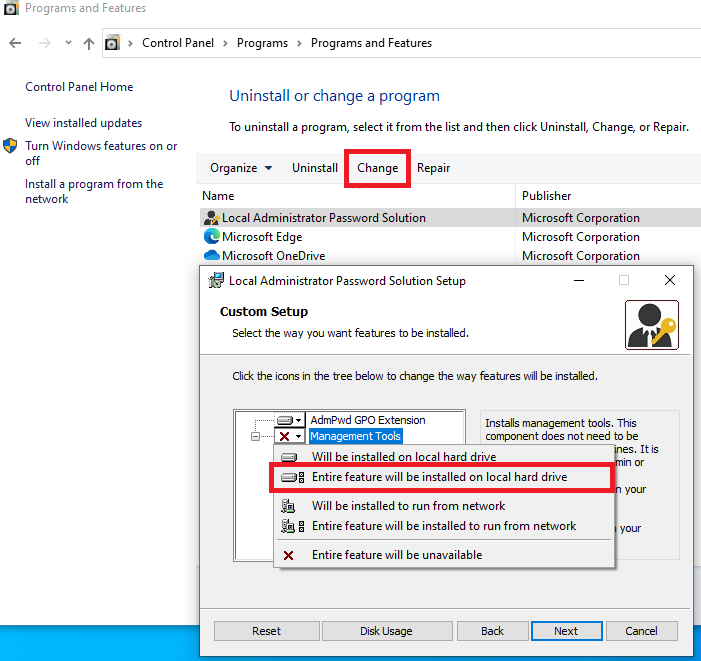
\includegraphics[width=0.7\linewidth]{../img/LAPS/laps-ui-install-2.png}
    \caption{LAPS GUI Installieren 2}
\end{figure}


\subsection{Active Directory vorbereiten}
Die zusätzlichen Extension Attributes können per Powershell hinzugefügt werden.
Der ausführende Domänenbenutzer muss ein ``Schema Admin'' in Active Directory sein.\\
\begin{figure}[H]
    \centering
    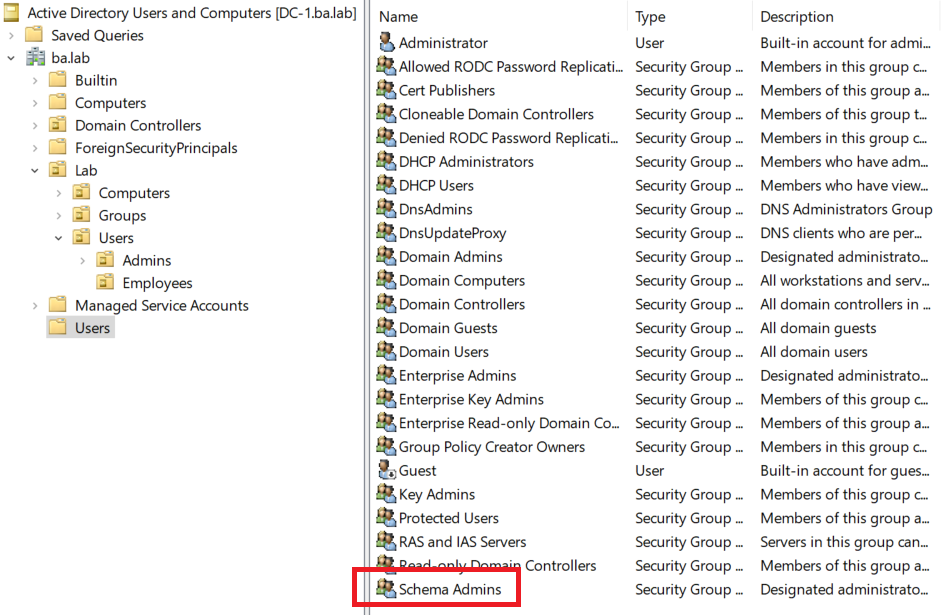
\includegraphics[width=0.7\linewidth]{../img/LAPS/schema-admins.png}
    \caption{Schema Admins Gruppe}
\end{figure}

Powershell mit dem Schema Admin Benutzer starten und folgendes Eingeben
\begin{lstlisting}
Import-module AdmPwd.PS
Update-AdmPwdADSchema

#Resultat:
#Operation            DistinguishedName                                              Status
#---------            -----------------                                              ------
#AddSchemaAttribute   cn=ms-Mcs-AdmPwdExpirationTime,CN=Schema,CN=Configuration,DC=b Success
#AddSchemaAttribute   cn=ms-Mcs-AdmPwd,CN=Schema,CN=Configuration,DC=ba,DC=lab       Success
#ModifySchemaClass    cn=computer,CN=Schema,CN=Configuration,DC=ba,DC=lab            Success

Set-AdmPwdComputerSelfPermission -OrgUnit "<Name der OU>"
#Resultat:
#Name                 DistinguishedName                                              Status
#----                 -----------------                                              ------
#Clients              OU=Clients,OU=Computers,OU=Lab,DC=ba,DC=lab                    Delegated
\end{lstlisting}

Nun muss noch eine Active Directory Gruppe erstellt werden.
Dieser Gruppe kann man alle Benutzer hinzufügen, welche Zugriff auf die Passwörter bekommen sollen.

\begin{figure}[H]
    \centering
    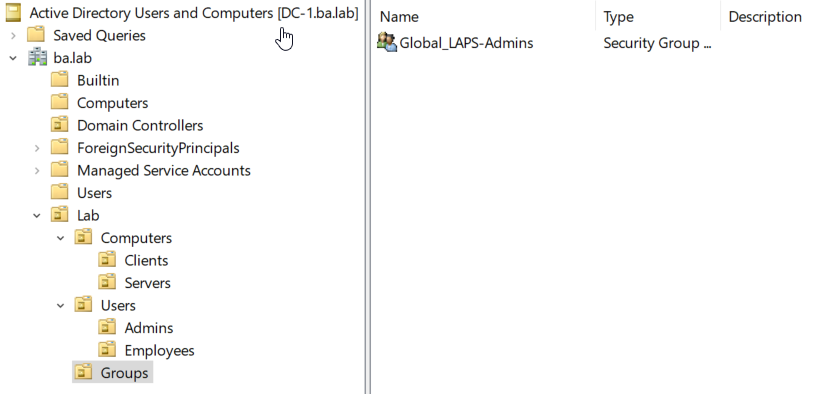
\includegraphics[width=\linewidth]{../img/LAPS/Laps-Admins.png}
    \caption{LAPS Active Directory Gruppe}
\end{figure}

Nach dem erstellen der Gruppe, muss zusätzlich noch eine Berechtigung auf der OU für die Gruppe eingerichtet werden.
Dazu muss ASEdit und die Eigenschaften der OU geöffnet werden. Im ``Security'' Tab
\begin{figure}[H]
    \centering
    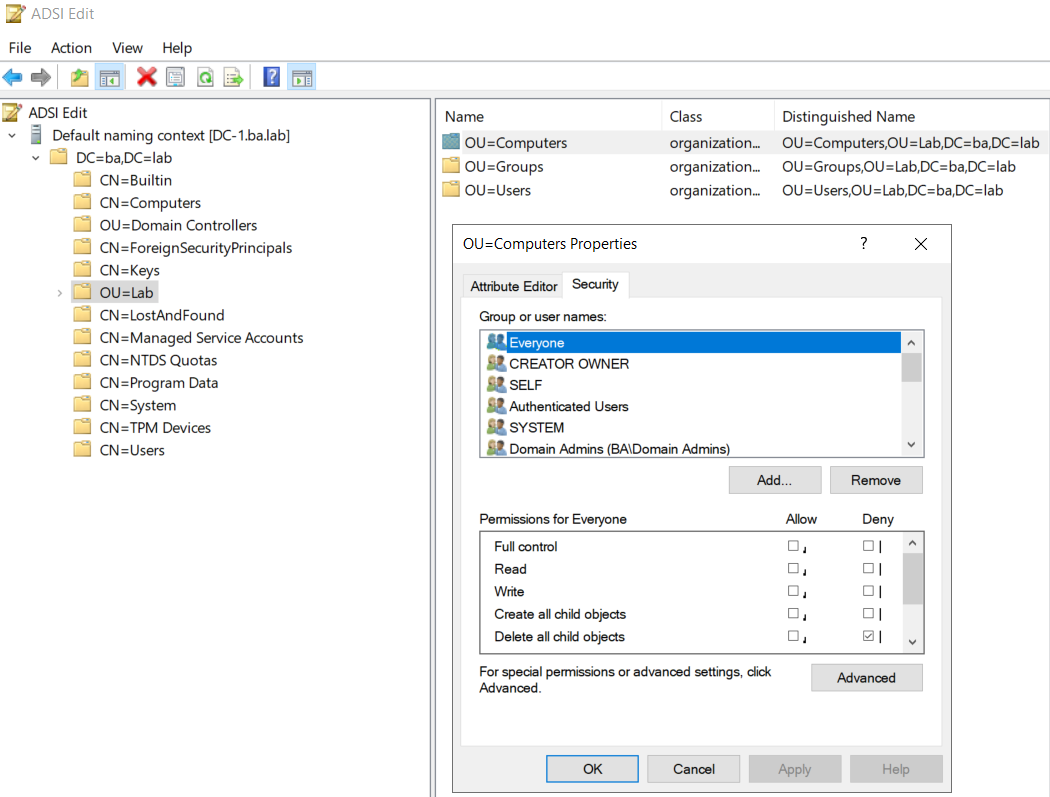
\includegraphics[width=0.7\linewidth]{../img/LAPS/ASEdit.png}
    \caption{ASEdit}
\end{figure}
unter ``Advanced'' muss die neue Gruppe hinzugefügt werden mit der Berechtigung ``All Extended Rights''.\\

Nun muss für LAPS noch die Verknüpfung zwischen dieser Gruppe und der OU erstellt werden.
Dies kann mit Powershell erledigt werden:
\begin{lstlisting}
Set-AdmPwdReadPasswordPermission -OrgUnit "<Name der OU>" -AllowedPrincipals Global_LAPS-Admins
Set-AdmPwdResetPasswordPermission -OrgUnit "<Name der OU>" -AllowedPrincipals Global_LAPS-Admins
\end{lstlisting}
Die Read Berechtigung erlaubt das Lesen der Passwörter.
Die Reset Berechtigung erlaubt das setzten eines Ablaufdatums eines Passwortes.
Die Berechtigung kann nun noch mii Powershell überprüft werden:
\begin{lstlisting}
Find-AdmPwdExtendedrights -identity "<Name der OU>"
\end{lstlisting}


\subsection{LAPS aktivieren}
Zum Schluss muss LAPS noch mit einer neuen Group Policy aktiviert werden.

Im Group Policy Management muss eine neue Group Policy erstellt werden, welche mit der gleichen OU verknüpft ist, wie die Group Policy für das Deployment.
\begin{figure}[H]
    \centering
    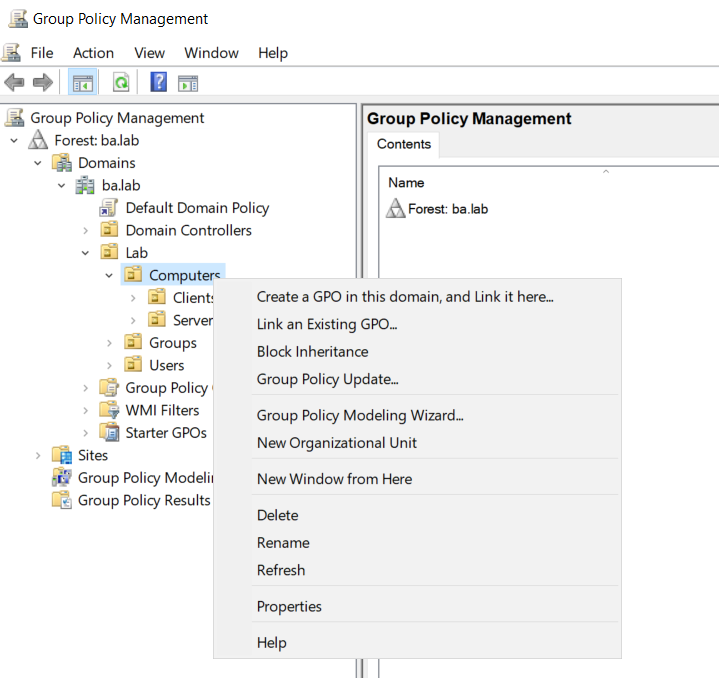
\includegraphics[width=0.7\linewidth]{../img/LAPS/GPO-Create-New.png}
    \caption{Neue GP für LAPS Deployment}
\end{figure}

Mit \textbf{Rechtsklick $\rightarrow$ Edit} kann die neue Group Policy bearbeitet werden.
Unter \textbf{Computer Configuration $\rightarrow$ Policies $\rightarrow$ Administrative Templates $\rightarrow$ Laps} findet man die Einstellungen von LAPS.
Mit \textbf{Rechtsklick $\rightarrow$ Edit} auf ``Enable local admin password management'' kann man die Einstellung öffnen und Links auf ``Enabled'' setzen.
Mit OK bestätigen.
\begin{figure}[H]
    \centering
    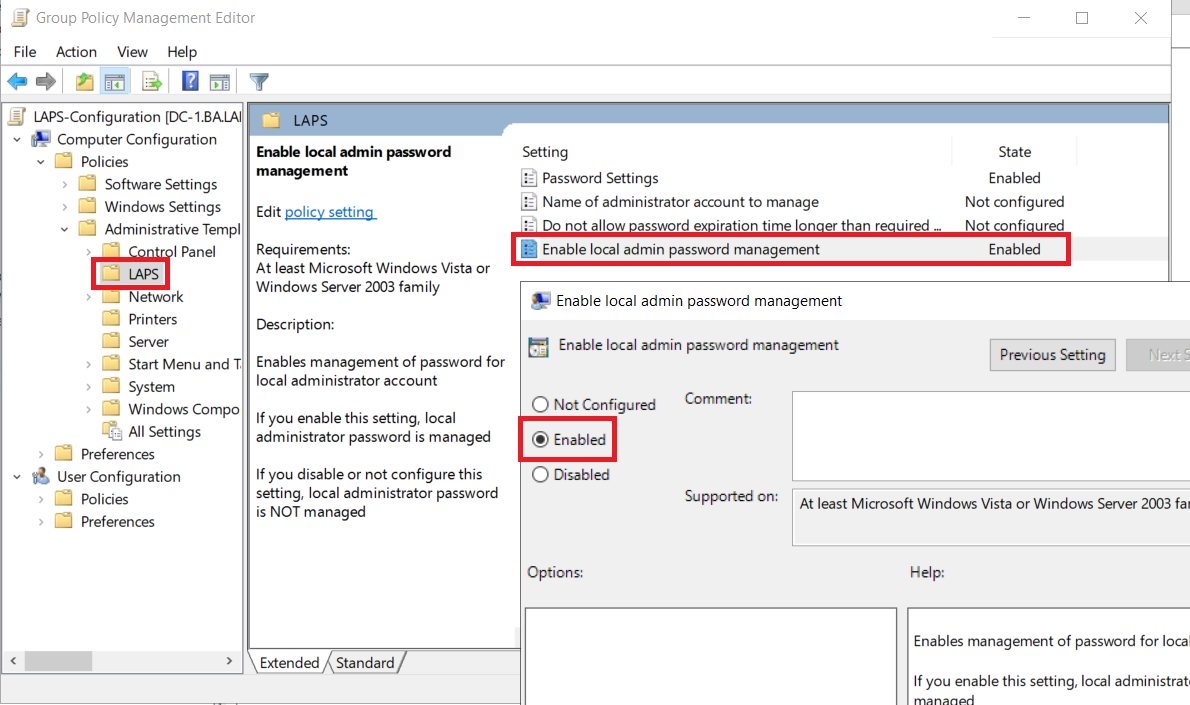
\includegraphics[width=0.7\linewidth]{../img/LAPS/enable-laps.png}
    \caption{LAPS aktivieren}
\end{figure}

In der Einstellung ``Password Settings'' kann man die Passwort Länge und den Zyklus setzten, wie oft das Passwort gewechselt werden soll.\\

Die Group Policy kann nun geschlossen werden.


\section{Verwendung}
\subsection{Mit dem GUI}\label{subsec:laps-gui-usage}
Das auslesen eines Passwortes über das GUI geht nur, wenn das GUI auch installiert wurde.
Die Installation des GUI wird im Kapitel \hyperref[subsubsec:Laps-Gui]{LAPS GUI für Admins} erklärt.\\

Im Startmenü muss man nach \textbf{LAPS UI} suchen. Falls der in Windows angemeldete Benutzer Berechtigung besitzt, LAPS Passwörter auszulesen, kann LAPS dirket gestartet werden.\\
Falls nicht, muss man den Speicherort der Datei öffnen.
Dann kann man mit \textbf{Shift + Rechtsklick} das Kontextmenü öffnen und die Datei mit ``Run as different user'' als anderen Benutzer ausführen.
Ein Eingabefenster öffnet sich, wo man den berechtigten Benutzer und das Passwort des Benutzer eingeben kann.
Berechtigt sind alle Benutzer in der zuvor erstellten Gruppe und Domänen Administratoren.\\
\begin{minipage}{0.5\linewidth}
    \begin{figure}[H]
        \centering
        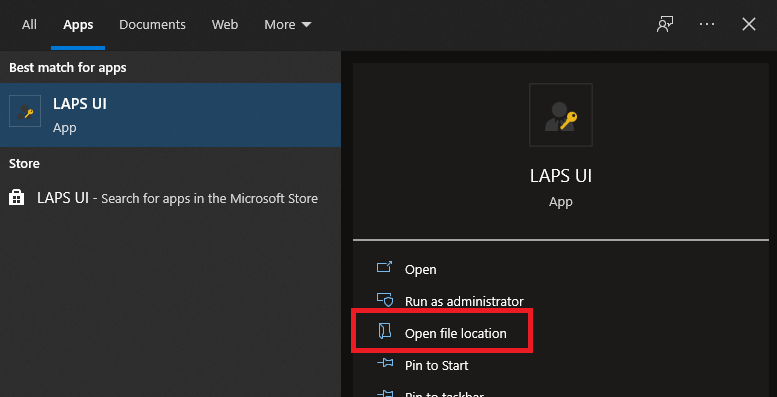
\includegraphics[width=\linewidth]{../img/LAPS/usage-1.png}
        \caption{LAPS Speicherort öffnen}
    \end{figure}
\end{minipage}
\begin{minipage}{0.5\linewidth}
    \begin{figure}[H]
        \centering
        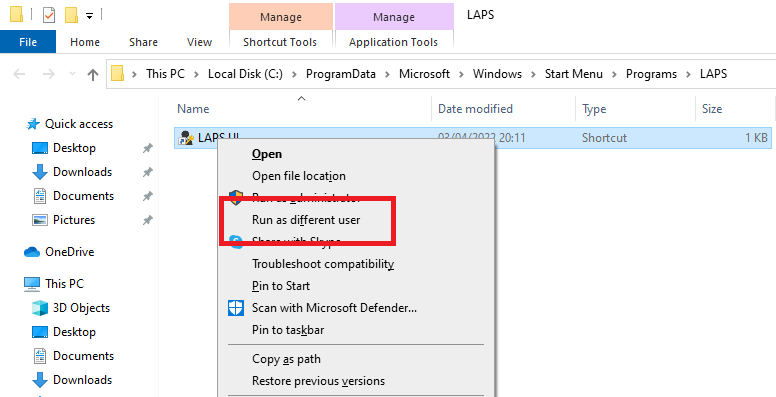
\includegraphics[width=\linewidth]{../img/LAPS/usage-2.png}
        \caption{LAPS als anderer Benutzer starten}
    \end{figure}
\end{minipage}\\

Im LAPS UI gibt man im Feld ``Computer name'' den Namen des Computers ein, von welchem man das lokale Passwort möchte.
Das Passwort wird dann im Feld ``Password'' angezeigt.
\begin{figure}[H]
    \centering
    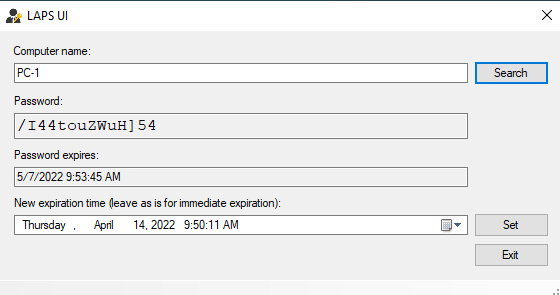
\includegraphics[width=0.7\linewidth]{../img/LAPS/Laps-ui.png}
    \caption{LAPS Passwort auslesen}
\end{figure}
Im Feld ``New expiration time'' kann man eine neue Zeit setzten, wann das Passwort gewechselt werden soll.

\subsection{Mit Powershell}
Die Powershell muss als Benutzer gestartet werden, welcher die Berechtigung hat das Passwort auszulesen oder zurückzusetzten.
Powershell als ein anderer Benutzer starten kann man gleich wie LAPS im Kapitel \hyperref[subsec:laps-gui-usage]{``Mit dem GUI''} als anderer Benutzer gestartet wurde.\\

Für das Auslesen und Zurücksetzen gibt es folgende Befehle:
\begin{lstlisting}
    Get-AdmPwdPassword -ComputerName <Computer Name>
    Reset-AdmPwdPassword -ComputerName <Computer Name>
\end{lstlisting}


\section{Best Practices}
Idealerweise sollten nur ausgewählte IT Mitarbeitende die Berechtigung erhalten, Passwörter auslesen zu können.
Alle Lokale Administratorrechte von AD Benutzern sollten entfernt werden und nur noch LAPS Passwörter verwendet werden.
Dadurch kann man verhindern, dass es einen Benutzer gibt, welcher auf allen Systemen berechtigt ist.\\

Falls ein Mitarbeitender ohne LAPS Berechtigung lokale Administratorrechte braucht, kann diesem das LAPS Paswort gegeben werden.
Dann sollte man aber auch das ``Expire Date'' auf das Datum setzten, wo das Passwort nicht mehr gebraucht wird.
Zum Beispeil am nächsten Tag.

\section{Intergration in Wazuh}
In Wazuh existiert eine Regel, welche jedes auslesen meldet.
Die Regel hat die ID 110010 und der Agent Name ist der \textbf{Domain Controller}.
Es ist nicht der der Computer, auf welchem das Passwort ausgelesen wurde.
\begin{figure}[H]
    \centering
    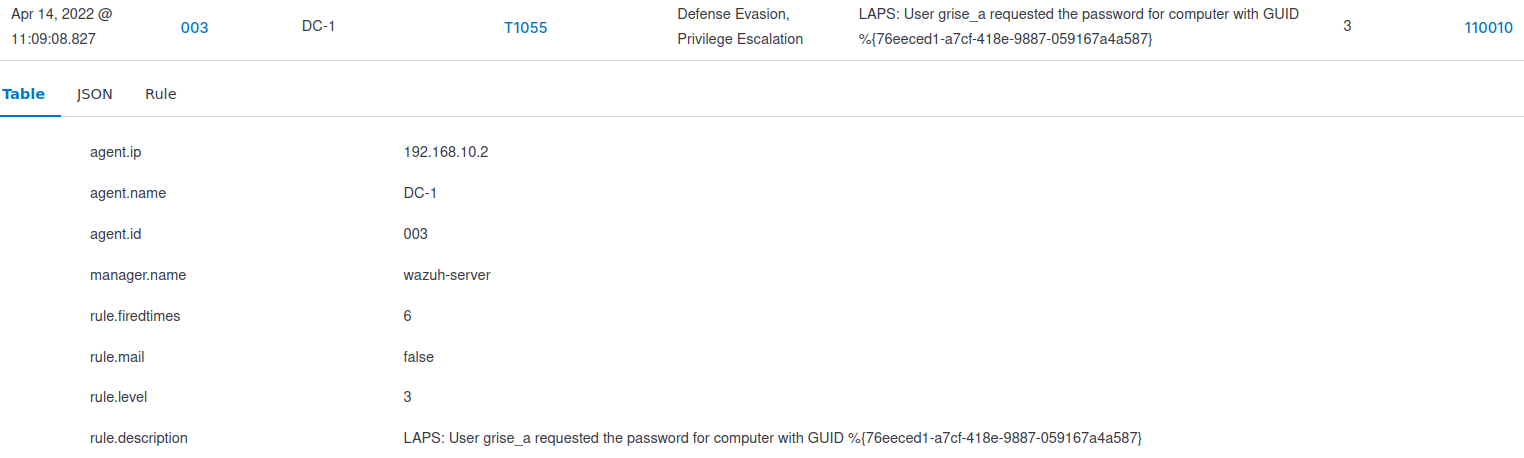
\includegraphics[width=\linewidth]{../img/LAPS/laps-wazuh.png}
    \caption{LAPS Wazuh Alert}
\end{figure}
Somit weiss man wer für welchen Computer das Passwort ausgelesen hat.
Man kann jedoch nicht feststellen, von welchem Computer aus das Passwort ausgelesen wurde.\\

Zusätzlich wird nur die GUID des Computers angezeigt, für welchen man das Passwort ausgelesen hat.
Um den Computernamen zu finden, kann man folgenden Powershell Befehl verwenden:
\begin{lstlisting}
    #GUID mit { } eingeben!
    Get-ADObject -Identity "<GUID>"
\end{lstlisting}

Zusätzlich gibt es noch eine Regel, welche einen Alert generiert, sobald 20 LAPS Passwörter in 10 Minuten ausgelesen wurden.
\begin{figure}[H]
    \centering
    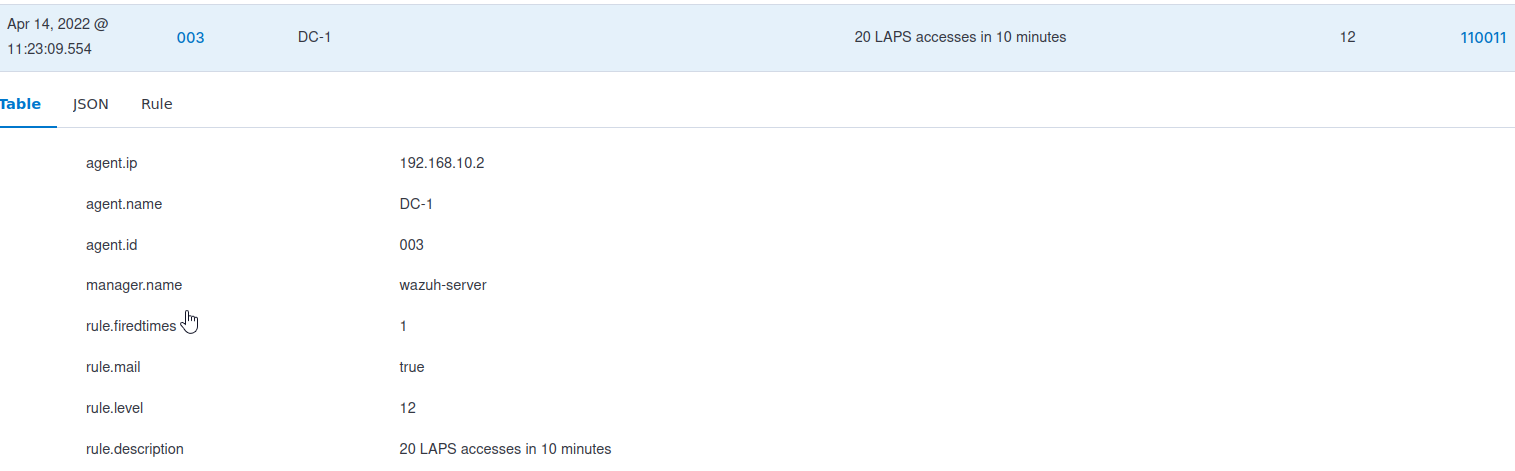
\includegraphics[width=\linewidth]{../img/LAPS/laps-wazuh-alert.png}
    \caption{LAPS Wazuh Alert 2}
\end{figure}